% THESIS_CHAPTER_MAP.tex
% Definitive mapping: SAMBP TRs → journal papers → thesis chapters
% Compile: pdflatex -> pdflatex
% Author: Anoop V. Eluvathingal | IITM EE | April 2026
%
% PURPOSE
% -------
% This document locks the thesis chapter structure before TR-56 (DFIG) begins.
% It prevents the "I have 9 papers but they don't form coherent chapters" problem
% by defining each chapter's UNIFYING PROBLEM, primary evidence, and sequencing.
%
% Once approved, this map governs:
%   (a) which new TRs to write vs skip
%   (b) which subsections belong in each chapter
%   (c) which journal paper maps to which chapter
%   (d) what the examiner reads as the chapter's claim

\documentclass[11pt, a4paper]{article}

\usepackage[T1]{fontenc}
\usepackage[utf8]{inputenc}
\usepackage[margin=22mm, top=20mm]{geometry}
\usepackage{amsmath, amssymb}
\usepackage{booktabs, array, multirow, tabularx, longtable}
\usepackage{graphicx}
\usepackage{xcolor}
\usepackage{hyperref}
\usepackage{pgfplots}
\pgfplotsset{compat=1.18}
\usepackage{tikz}
\usetikzlibrary{arrows.meta, positioning, calc, fit, backgrounds,
                shapes.geometric, matrix, decorations.pathreplacing}
\usepackage{caption}
\usepackage{parskip}
\usepackage{enumitem}
\usepackage{colortbl}
\usepackage{rotating}

\hypersetup{colorlinks=true, linkcolor=blue!60!black, citecolor=blue!60!black}

% ---- Colour palette -----------------------------------------------------------
\definecolor{C1col}{RGB}{0,70,140}      % Ch2: Machine Modelling
\definecolor{C2col}{RGB}{0,120,60}      % Ch3: OC Protection
\definecolor{C3col}{RGB}{150,60,0}      % Ch4: Line Differential
\definecolor{C4col}{RGB}{100,0,120}     % Ch5: Transformer Diff
\definecolor{C5col}{RGB}{160,0,30}      % Ch6: Generator Suite
\definecolor{C6col}{RGB}{0,100,130}     % Ch7: System Integration
\definecolor{donecol}{RGB}{0,140,60}
\definecolor{wip}{RGB}{200,120,0}
\definecolor{planned}{RGB}{120,120,120}
\definecolor{warningred}{RGB}{180,0,0}

\newcommand{\done}[1]{\textcolor{donecol}{\textbf{#1}}}
\newcommand{\wipp}[1]{\textcolor{wip}{#1}}
\newcommand{\plan}[1]{\textcolor{planned}{\textit{#1}}}

\newcommand{\chap}[2]{\noindent\textbf{\color{#1}#2}}
\newcommand{\chtag}[2]{\colorbox{#1}{\color{white}\textbf{\small #2}}}

\setlength{\tabcolsep}{5pt}
\renewcommand{\arraystretch}{1.15}

\title{\textbf{PhD Thesis Chapter Map}\\[4pt]
       \large Smart Adaptive Multi-Bus Protection (SAMBP) for IBR Networks\\[2pt]
       \normalsize Version 1.0 — Locked April 2026}
\author{Anoop V. Eluvathingal \quad|\quad IIT Madras, EE Department}
\date{April 2026}

% ==============================================================================
\begin{document}
\maketitle

\noindent\fbox{\parbox{\dimexpr\linewidth-2\fboxsep\relax}{\small
\textbf{Lock purpose:} This map is frozen before TR-56 (DFIG) begins.  Any new TR
must declare its chapter home before development starts.  Each chapter is defined
by a \emph{unifying problem statement} — not a collection of methods — so the
examiner reads a coherent argument, not a catalogue.}}

\tableofcontents
\clearpage

% ==============================================================================
\section{Thesis Identity and Central Claim}
\label{sec:identity}

\subsection{One-Sentence Thesis}

\begin{center}
\fbox{\parbox{0.90\linewidth}{\centering\large
\textit{Existing protection elements for lines, transformers, and generators fail
in IBR-dominated grids because they were parametrised on synchronous-machine fault
physics; a unified model-based inference framework re-parametrises each element
from the measurable IBR current envelope, restoring protection reliability without
replacing field hardware.}}}
\end{center}

\subsection{Three-Layer Architecture}

Every chapter's contribution maps to one of three architectural layers:

\begin{center}
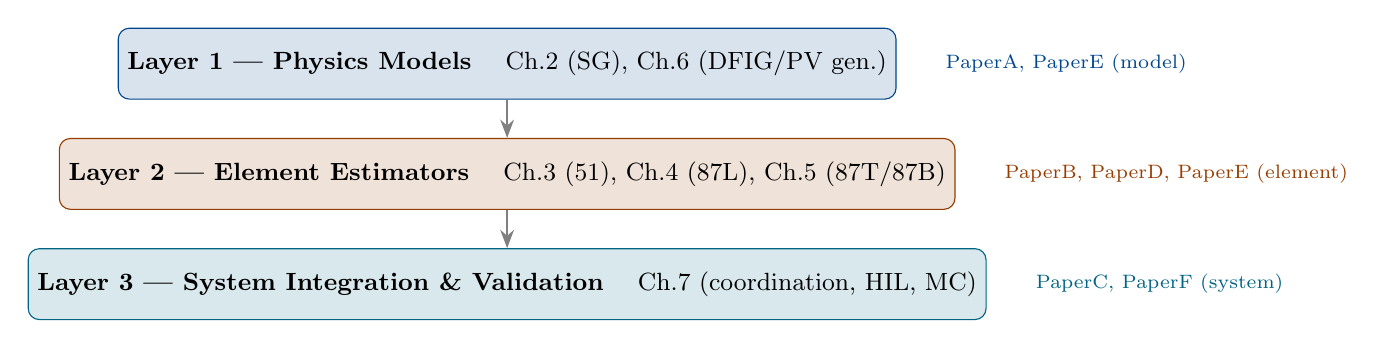
\begin{tikzpicture}[
  box/.style={rectangle, draw, rounded corners, minimum width=8cm,
              minimum height=0.9cm, align=center, font=\small},
  arr/.style={-Stealth, thick, gray},
]
\node[box, fill=C1col!15, draw=C1col] (L1) at (0,0)
  {\textbf{Layer 1 — Physics Models}
  \quad Ch.2 (SG), Ch.6 (DFIG/PV gen.)};
\node[box, fill=C3col!15, draw=C3col] (L2) at (0,-1.4)
  {\textbf{Layer 2 — Element Estimators}
  \quad Ch.3 (51), Ch.4 (87L), Ch.5 (87T/87B)};
\node[box, fill=C6col!15, draw=C6col] (L3) at (0,-2.8)
  {\textbf{Layer 3 — System Integration \& Validation}
  \quad Ch.7 (coordination, HIL, MC)};
\draw[arr] (L1) -- (L2);
\draw[arr] (L2) -- (L3);
\node[right=0.5cm of L1, font=\scriptsize, C1col] {PaperA, PaperE (model)};
\node[right=0.5cm of L2, font=\scriptsize, C3col] {PaperB, PaperD, PaperE (element)};
\node[right=0.5cm of L3, font=\scriptsize, C6col] {PaperC, PaperF (system)};
\end{tikzpicture}
\end{center}

% ==============================================================================
\section{Chapter Structure Overview}
\label{sec:overview}

\begin{table}[!h]
\centering
\caption{Thesis Chapters at a Glance}
\label{tab:overview}
\begin{tabular}{clp{5.5cm}cp{2.8cm}c}
\toprule
Ch. & Title & Unifying Problem & Pages & Primary papers & Status \\
\midrule
1 & Introduction & IBR breaks all protection & 25 & --- & \done{Draft} \\
\rowcolor{C1col!8}
2 & Machine Modelling & Relay needs reduced model & 30 & PaperA, PaperE§II--III & \done{Done} \\
\rowcolor{C2col!8}
3 & OC Protection & 51 miscoordinates for IBR & 35 & PaperE, PaperB & \done{Done} \\
\rowcolor{C3col!8}
4 & Line Differential & 87L blind below $k_{\rm ibr}$ & 45 & PaperD, TR-62 & \done{Done} \\
\rowcolor{C4col!8}
5 & Transformer Diff & 2nd harm. blocks IBR faults & 35 & TR-57, TR-64, PaperC§IV & \wipp{Q3 2026} \\
\rowcolor{C5col!8}
6 & Generator Suite & 40/64G/78/81/87G fail IBR & 50 & TR-56--65 & \plan{Q1 2028} \\
\rowcolor{C6col!8}
7 & System Integration & Elements don't coordinate & 30 & PaperC, PaperF, TR-66/67 & \plan{Q2 2028} \\
8 & Conclusions & --- & 15 & --- & \plan{Q3 2028} \\
\midrule
\multicolumn{3}{r}{\textbf{Total (excl. Ch.1, Ch.8)}} & \textbf{225} & & \\
\bottomrule
\end{tabular}
\end{table}

% ==============================================================================
\section{Chapter-by-Chapter Specifications}
\label{sec:chapters}

% ------------------------------------------------------------------------------
\subsection{Chapter 1: Introduction}

\textbf{Function:} Frame the problem, survey the field, state thesis contributions.
Not a data chapter — examiner does not evaluate claims here.

\textbf{Must contain:}
\begin{itemize}[nosep]
  \item One-paragraph statement of each IBR protection failure mode (5 types)
  \item Literature review table: per protection element, current best method, its failure mode, how this thesis addresses it
  \item Contribution list that maps 1:1 to Chapters 2--7
  \item Chapter dependency diagram (same as Figure~\ref{fig:dep} below)
\end{itemize}

\textbf{Sources:} No original results. Cite all existing papers once each.

% ------------------------------------------------------------------------------
\subsection{Chapter 2: Machine Modelling for Protection}

\chtag{C1col}{Layer 1} \quad \textbf{Target journal: IEEE Transactions on Energy Conversion (PaperA)}

\textbf{Unifying problem:} Protection relays use simplified machine models
(constant-voltage-behind-subtransient-reactance) that fail to predict fault
current amplitude and decay for both synchronous generators and IBRs.  Without
a correct model the estimator in every subsequent chapter cannot converge.

\textbf{Narrative arc:}
\begin{enumerate}[nosep]
  \item 6th-order Park dq model as the truth model (§2.1--2.2)
  \item Reduction to 4-parameter relay model via AVR dominance argument (§2.3)
  \item Validation: reduced model error $< 5\%$ for $L^* \leq 150\,\text{ms}$ (§2.4)
  \item IBR equivalent: PV gives 2-param sinusoid; DFIG gives 3-param (§2.5 — preliminary, full in Ch.6)
\end{enumerate}

\textbf{Primary evidence:}
\begin{itemize}[nosep]
  \item PaperA (ieee\_6th\_order): full 6th-order model + validation, 18 figures
  \item PaperE §II--III: reduced model derivation and LM estimator
\end{itemize}

\textbf{TRs that feed this chapter:}
\begin{center}
\begin{tabular}{ll}
\toprule
TR & Contribution to Ch.2 \\
\midrule
sync\_oc/report1--3 & SG mathematical model development \\
sync\_oc/report4--5 & Reduced 4-param model identifiability \\
TR-56 (planned) & DFIG 10-param ODE → preliminary 3-param relay model \\
\bottomrule
\end{tabular}
\end{center}

\textbf{Chapter closes with:} A model taxonomy table (SG 4-param, PV 2-param, DFIG 3-param)
that is referenced by all subsequent chapters when citing their zone model.

% ------------------------------------------------------------------------------
\subsection{Chapter 3: IBR-Adaptive Overcurrent Protection (Relay 51)}

\chtag{C2col}{Layer 2} \quad \textbf{Target journals: IEEE TPWRD (PaperE), IEEE TPWRD (PaperB)}

\textbf{Unifying problem:} The inverse-time overcurrent relay (ANSI 51) selects
$I_p$ and TMS by fitting an IEC curve to the pre-fault SG impedance.  When IBRs
feed the bus, fault current is limited to $k_{\rm ibr} < I_p$, causing the relay
to either fail to pick up or miscoordinate with upstream devices.

\textbf{Narrative arc:}
\begin{enumerate}[nosep]
  \item Failure modes: blinding ($k_{\rm ibr} < I_p$), sympathetic tripping ($\phi$ mismatch) (§3.1)
  \item Two-pass LM estimator for SG-sourced 51: identifies $\{I_p, \text{TMS}\}$ from fault transient (§3.2--3.3)
  \item Confidence gate and adaptive parameter update (§3.4)
  \item Milestone 1 results: 12/12 SG fault scenarios, TMS adaptation (§3.5)
  \item High-impedance fault sensitivity: TMS floor at $\text{TMS}_{\min}=0.050$ (§3.6)
  \item PaperB: HIF identification on mixed SG+IBR bus, coordination implications (§3.7--3.8)
\end{enumerate}

\textbf{Primary evidence:}
\begin{itemize}[nosep]
  \item PaperE (sambp\_sync\_oc/paper): complete, 8pp, Milestone 1+2 data
  \item PaperB (ieee\_hif\_tpwd): complete, 9pp
\end{itemize}

\textbf{TRs that feed this chapter:}
\begin{center}
\begin{tabular}{ll}
\toprule
TR & Contribution to Ch.3 \\
\midrule
sync\_oc/report1--6 & Zone model, LM passes, confidence gate \\
hif\_paper reports & HIF current model on SG bus, coordination \\
\bottomrule
\end{tabular}
\end{center}

\textbf{Key limitation stated in this chapter:} TMS is clamped at
$\text{TMS}_{\min}$ for all HIF cases — a coordination-level constraint, not
an estimator limitation.  This motivates Chapter 7 (system coordination).

\textbf{What this chapter does NOT cover:}
IBR-sourced OC adaptation (DFIG or PV feeding fault) is deferred to Chapter 6
(generator protection suite), where the DFIG model is derived first.

% ------------------------------------------------------------------------------
\subsection{Chapter 4: IBR-Tolerant Line Current Differential Protection (87L)}

\chtag{C3col}{Layer 2} \quad \textbf{Target journal: IEEE Transactions on Industrial Electronics (PaperD)}

\textbf{Unifying problem:} The fixed-threshold 87L is blind to internal faults when
$k_{\rm ibr} < I_{\rm op,min} = 0.20\,\text{pu}$.  No single fix suffices:
the threshold must adapt, negative sequence must be added for SLG faults,
zero-sequence must handle pure-IBR earth faults, a transient element must detect
symmetric 3-phase faults below the threshold, and the zone model must handle PV
(zero DC) vs.\ SG (DC exponential) differently.

\textbf{This chapter has the strongest evidence base of the thesis}
(21 deterministic + 15\,000 MC scenarios, two published TRs, one complete journal paper).

\textbf{Narrative arc:}
\begin{enumerate}[nosep]
  \item Problem: $k_{\rm ibr}$ detection floor and the 5 failure modes (§4.1)
  \item Adaptive threshold law: $I_{\rm thr} = \max(0.08, 0.15 I_{\rm rest})$ → 30$\times$ CT margin (§4.2)
  \item 87LN element: negative sequence for SLG under IBR (§4.3)
  \item 87LN0 element: zero-sequence 87L for pure-IBR earth faults (§4.4)
  \item TDCS element: transient differential for 3-phase IBR faults, floor 0.058 pu (§4.5)
  \item PV zone model: 2-param, $\kappa_n=1$, 36$\times$ condition number improvement (§4.6)
  \item $k_{\rm ibr}$-driven model selector: DDR criterion, delta-ratio veto (§4.7)
  \item Full 21-scenario results and 15k MC (§4.8)
\end{enumerate}

\textbf{Primary evidence:}
\begin{itemize}[nosep]
  \item PaperD (ieee\_line\_diff): complete, 9pp, all elements integrated
  \item TR-62 (sambp/report62): PV zone model, 9pp, Python modules
\end{itemize}

\textbf{TRs that feed this chapter:}
\begin{center}
\begin{tabular}{ll}
\toprule
TR & Contribution to Ch.4 \\
\midrule
TR-10--12 & CT saturation, magnitude override, charging compensation \\
TR-13, 15 & Pi-section model, voltage correction \\
TR-17 & Adaptive threshold law \\
TR-20 & Frequency-adaptive charging current \\
TR-22 & 87LN negative-sequence element \\
TR-23 & TDCS element, 0.058 pu floor derivation \\
TR-24 & Adaptive TDCS threshold for drifting baseline \\
TR-25 & 87LN0 zero-sequence element \\
TR-26 & IBR parametric Monte Carlo (15k trials, TR-26 parametric) \\
TR-27 & Monte Carlo robustness study \\
TR-62 & PV 2-parameter zone model + $k_{\rm ibr}$ selector \\
\bottomrule
\end{tabular}
\end{center}

\textbf{Boundary with Ch.5:} The 87L detects line faults; the 87T detects
transformer internal faults.  The charging current compensation (§4.2) is
distinct from the inrush restraint problem (Ch.5).

% ------------------------------------------------------------------------------
\subsection{Chapter 5: IBR-Tolerant Transformer Differential Protection (87T)}

\chtag{C4col}{Layer 2} \quad \textbf{Target journal: IEEE Transactions on Power Delivery}

\textbf{Unifying problem:} The IEC 60255-111 / IEEE C37.91 mandate of 2nd-harmonic
restraint fails in two directions in IBR networks:
(a) IBR fault current is inherently low in harmonic content ($I_{2f}/I_{1f}$
below restraint threshold) → security failure (refuses to trip on genuine fault);
(b) deep core saturation from large inrush reduces 2nd harmonic below threshold
→ dependability failure (trips on inrush).

\textbf{Narrative arc:}
\begin{enumerate}[nosep]
  \item IBR fault current harmonic spectrum: PR controller bandwidth argument (§5.1)
  \item Failure modes of 2nd-harmonic restraint with IBR source (§5.2)
  \item Waveform asymmetry index $A_k$: physical basis, three hypotheses (§5.3)
  \item Jiles--Atherton derivation of $H_0$ distribution: $\mathcal{TN}(+0.70, 0.15^2)$ (§5.4)
  \item IBR symmetry constraint: $H_1$ distribution $\mathcal{TN}(0.00, 0.08^2)$ (§5.5)
  \item CT saturation asymmetry: $H_2$ distribution $\mathcal{TN}(-0.50, 0.20^2)$ (§5.6)
  \item SPRT: Wald boundaries $\pm 6.91$, KL divergence $D_{\rm KL}=11.17$ nats (§5.7)
  \item Decision time: 20\,ms vs.\ $\geq 60$\,ms for 2nd-harmonic method (§5.8)
  \item Integration with SAMBP 87T Stage-2 gate (§5.9)
  \item Simulation results: 24 deterministic + 5k MC (§5.10) [TR-64 deliverable]
\end{enumerate}

\textbf{Primary evidence:}
\begin{itemize}[nosep]
  \item TR-57 (sambp/report57): complete, 14pp, full mathematical derivation
  \item TR-64 (planned Q2--Q3 2027): simulation study, PSCAD validation
  \item PaperC (ieee\_seq\_estim) §IV: sequence estimator applied to 87T cross-check
  \item Existing SAMBP 87T work (TR-30 area): LM estimator for 87T (background)
\end{itemize}

\textbf{TRs that feed this chapter:}
\begin{center}
\begin{tabular}{ll}
\toprule
TR & Contribution to Ch.5 \\
\midrule
TR-30--45 (area) & SAMBP 87T LM estimator, inrush, CT saturation baseline \\
TR-57 & SPRT asymmetry inrush restraint (complete) \\
TR-64 (planned) & Full 87T+SPRT integration, 5k MC \\
\bottomrule
\end{tabular}
\end{center}

\textbf{Standards challenge:} This chapter explicitly challenges IEC 60255-111.
The examiner will ask: ``Have you submitted a standards comment?''  The answer
is ``A proposal for IEC TC95 is prepared as a companion deliverable after TR-64.''

% ------------------------------------------------------------------------------
\subsection{Chapter 6: Generator Protection Suite for IBR Networks}
\label{sec:ch6}

\chtag{C5col}{Layer 1+2} \quad \textbf{Target journals: IEEE TEC (TR-56), IEEE TPWRS (TR-58), IEEE TPWRD (TR-60), IEEE TIE (TR-61)}

\textbf{Unifying problem:} The five standard generator protection functions
(40/64G/78/81/87G) were designed assuming the generator is directly connected
to an SG-dominated network.  When the generator is an IBR (DFIG or PV) or when
the network becomes IBR-dominated, each function fails by a different mechanism:
\begin{itemize}[nosep]
  \item \textbf{Relay 40 (LOE):} Admittance locus shifts when GFM IBRs provide reactive support → spurious operation
  \item \textbf{Relay 64G (stator EF):} Sub-harmonic injection frequency must adapt to network impedance changes from IBRs
  \item \textbf{Relay 78 (out-of-step):} Equal-area criterion (EAC) breaks down for hybrid SG+GFM topology
  \item \textbf{Relay 81 (frequency):} ROCOF-based IFDI misfires in zero-inertia GFM networks
  \item \textbf{Relay 87G (gen.\ diff.):} DFIG rotor CTs are expensive or unavailable
\end{itemize}

\textbf{This chapter is the thesis's most novel contribution} — no prior work
addresses all five functions together under a unified IBR-correction framework.

\textbf{Narrative arc:}
\begin{enumerate}[nosep]
  \item DFIG and PV machine models for protection (§6.1) [TR-56]
  \item Virtual 87G-DFIG: slip-frequency EKF, no rotor CTs (§6.2) [TR-59]
  \item Relay 40 LOE: GFM IBR admittance correction (§6.3) [TR-60]
  \item Relay 64G: optimal sub-harmonic injection $f^*=25$--$35\,\text{Hz}$ (§6.4) [TR-61]
  \item Relay 78: generalised EAC for hybrid SG+GFM via Lyapunov (§6.5) [TR-58]
  \item Relay 81: IFDI for zero-inertia GFM networks (§6.6) [TR-63]
  \item Comprehensive suite: coordinated 40/64G/78/81/87G (§6.7) [TR-65]
\end{enumerate}

\textbf{TRs that feed this chapter:}
\begin{center}
\begin{tabular}{lll}
\toprule
TR & Topic & Target journal \\
\midrule
TR-56 (Q2--Q3 2026) & DFIG piecewise-ODE, CUSUM crowbar detection & IEEE TEC \\
TR-58 (Q2--Q3 2026) & Generalised EAC, IBR-corrected Relay 78 & IEEE TPWRS \\
TR-59 (Q4 2026) & Virtual 87G-DFIG via slip-frequency EKF & IEEE TEC \\
TR-60 (Q4 2026) & Relay 40 LOE + GFM IBR admittance correction & IEEE TPWRD \\
TR-61 (Q4 2026) & Relay 64G stator EF, optimal $f^*$ injection & IEEE TIE \\
TR-63 (Q2--Q3 2027) & Relay 81 IFDI for zero-inertia GFM & IEEE TSG \\
TR-65 (Q4 2027) & Comprehensive SG/DFIG/PV protection relay & IEEE TPWRD \\
TR-66 (Q4 2027) & 10k-trial MC per element & (internal) \\
\bottomrule
\end{tabular}
\end{center}

\textbf{Chapter opens with a coherence bridge from Ch.3:}
Overcurrent (Ch.3) addresses network-fed faults on SG buses.
Generator protection (Ch.6) addresses faults \emph{within} the generator itself
and loss of stable operation — a distinct physical problem.

% ------------------------------------------------------------------------------
\subsection{Chapter 7: System Integration and Validation}

\chtag{C6col}{Layer 3} \quad \textbf{Target journal: IEEE Transactions on Power Systems (PaperC/PaperF)}

\textbf{Unifying problem:} Each element (Ch.3--6) is validated independently.
But protection must \emph{coordinate}: an internal line fault must not cause a
generator trip; a loss-of-excitation event must not be confused with a busbar
fault.  System-level validation requires HIL with real relay hardware.

\textbf{Narrative arc:}
\begin{enumerate}[nosep]
  \item Sequence estimator as a cross-element inference backbone (§7.1--7.2) [PaperC]
  \item Unified SAMBP framework: IEC 61850 GOOSE coordination between elements (§7.3) [PaperF]
  \item N-1 coordination study: verify no misoperation between Ch.3--6 elements (§7.4) [TR-66]
  \item HIL validation: RTDS with DFIG+PV emulators, real relay hardware (§7.5) [TR-67]
  \item Performance summary across all elements vs.\ conventional (§7.6)
\end{enumerate}

\textbf{Primary evidence:}
\begin{itemize}[nosep]
  \item PaperC (ieee\_seq\_estim): complete, 9pp
  \item PaperF (paper\_c): complete, 6pp
  \item TR-67 (planned Q1--Q2 2028): HIL
\end{itemize}

\textbf{Key constraint:} Ch.7 cannot be completed before all elements in Ch.3--6
are available for the N-1 coordination study.  TR-65 (Q4 2027) is the
critical path item.

% ==============================================================================
\section{TR-to-Chapter Allocation}
\label{sec:allocation}

\begin{longtable}{lp{6.5cm}ccc}
\caption{Complete TR → Chapter allocation register}\label{tab:alloc}\\
\toprule
TR & Topic & Ch. & Status & Journal \\
\midrule
\endfirsthead
\multicolumn{5}{c}{\textit{(continued)}}\\
\toprule
TR & Topic & Ch. & Status & Journal \\
\midrule
\endhead
\bottomrule
\endfoot
% SG modelling
sync\_oc/R1--3 & SG zone model derivation & 2 & \done{Done} & PaperA \\
sync\_oc/R4--6 & Reduced model identifiability, LM & 2+3 & \done{Done} & PaperE \\
% OC protection
sync\_oc/R7+ & Milestone 1+2 data, HIF sweep & 3 & \done{Done} & PaperE \\
hif\_paper & HIF detection on SG+IBR bus & 3 & \done{Done} & PaperB \\
% 87L suite
TR-10 & CT saturation injection & 4 & \done{Done} & PaperD \\
TR-11 & HIF sensitivity margin & 4 & \done{Done} & PaperD \\
TR-12 & Magnitude override for 87L & 4 & \done{Done} & PaperD \\
TR-13 & Pi-section charging compensation & 4 & \done{Done} & PaperD \\
TR-15 & Voltage-based Pi-section correction & 4 & \done{Done} & PaperD \\
TR-16 & 87B/87L coordination & 4+7 & \done{Done} & PaperD/F \\
TR-17 & Adaptive threshold law & 4 & \done{Done} & PaperD \\
TR-18 & Mho distance relay (21/21P) & 4 (background) & \done{Done} & --- \\
TR-20 & Frequency-adaptive charging correction & 4 & \done{Done} & PaperD \\
TR-21 & Harmonic discrimination for 87L & 4 & \done{Done} & PaperD \\
TR-22 & 87LN negative-sequence element & 4 & \done{Done} & PaperD \\
TR-23 & TDCS element, 0.058 pu floor & 4 & \done{Done} & PaperD \\
TR-24 & Adaptive TDCS threshold & 4 & \done{Done} & PaperD \\
TR-25 & 87LN0 zero-sequence element & 4 & \done{Done} & PaperD \\
TR-26 & IBR parametric MC (15k) & 4 & \done{Done} & PaperD \\
TR-27 & MC robustness study & 4 & \done{Done} & PaperD \\
TR-62 & PV 2-param zone model + selector & 4 & \done{Done} & PaperD (§III update) \\
% 87T
TR-30--45 & 87T LM estimator + baseline & 5 & \done{Done} & (Ch.5 background) \\
TR-46--55 & 87T confidence gate, SPRT prep & 5 & \done{Done} & (Ch.5 background) \\
TR-57 & 3-hypothesis SPRT, Jiles--Atherton & 5 & \done{Done} & IEEE TPWRD \\
TR-64 (plan) & 87T+SPRT integration, 5k MC & 5 & \plan{Q2--Q3 2027} & IEEE TPWRD \\
% Generator suite
TR-56 (plan) & DFIG 10-param ODE, CUSUM & 6 & \plan{Q2--Q3 2026} & IEEE TEC \\
TR-58 (plan) & EAC Lyapunov, Relay 78 IBR & 6 & \plan{Q2--Q3 2026} & IEEE TPWRS \\
TR-59 (plan) & Virtual 87G-DFIG EKF & 6 & \plan{Q4 2026} & IEEE TEC \\
TR-60 (plan) & Relay 40 LOE + GFM correction & 6 & \plan{Q4 2026} & IEEE TPWRD \\
TR-61 (plan) & Relay 64G sub-harmonic injection & 6 & \plan{Q4 2026} & IEEE TIE \\
TR-63 (plan) & Relay 81 IFDI zero-inertia & 6 & \plan{Q2--Q3 2027} & IEEE TSG \\
TR-65 (plan) & Comprehensive gen.\ suite & 6 & \plan{Q4 2027} & IEEE TPWRD \\
TR-66 (plan) & 10k-trial MC per element & 6+7 & \plan{Q4 2027} & (internal) \\
% Integration
TR-67 (plan) & HIL with RTDS+DFIG+PV & 7 & \plan{Q1--Q2 2028} & (internal) \\
\end{longtable}

% ==============================================================================
\section{Journal Paper → Chapter Map}
\label{sec:papers}

\begin{table}[!h]
\centering
\caption{Six Journal Papers and Their Thesis Chapter Homes}
\label{tab:papers}
\begin{tabular}{llp{4.5cm}cc}
\toprule
Paper & File & Title (short) & Ch. & Target \\
\midrule
PaperA & ieee\_6th\_order & 6th-order Park dq validation & 2 & IEEE TEC \\
PaperB & ieee\_hif\_tpwd & HIF on IBR bus & 3 & IEEE TPWRD \\
PaperC & ieee\_seq\_estim & Sequence estimator framework & 7 & IEEE TPWRS \\
PaperD & ieee\_line\_diff & IBR-adaptive 87L suite & 4 & IEEE TIE \\
PaperE & sambp\_sync\_oc/paper & SG OC inverse estimation & 3 & IEEE TPWRD \\
PaperF & sambp\_sync\_oc/paper\_c & SAMBP unified framework & 7 & IEEE TPS \\
\bottomrule
\end{tabular}
\end{table}

\noindent\textbf{Chapter coverage check:}
\begin{itemize}[nosep]
  \item Ch.2 → primary: PaperA; secondary: PaperE §II--III
  \item Ch.3 → primary: PaperE + PaperB
  \item Ch.4 → primary: PaperD + TR-62
  \item Ch.5 → primary: TR-57 + TR-64; secondary: PaperC §IV
  \item Ch.6 → primary: TR-56/58/59/60/61/63/65 (journal papers each)
  \item Ch.7 → primary: PaperC + PaperF + TR-67
\end{itemize}

Every chapter has at least one published/complete primary source.
No chapter relies entirely on planned work.

% ==============================================================================
\section{Dependency and Critical Path}
\label{sec:dependency}

\begin{figure}[!h]
\centering
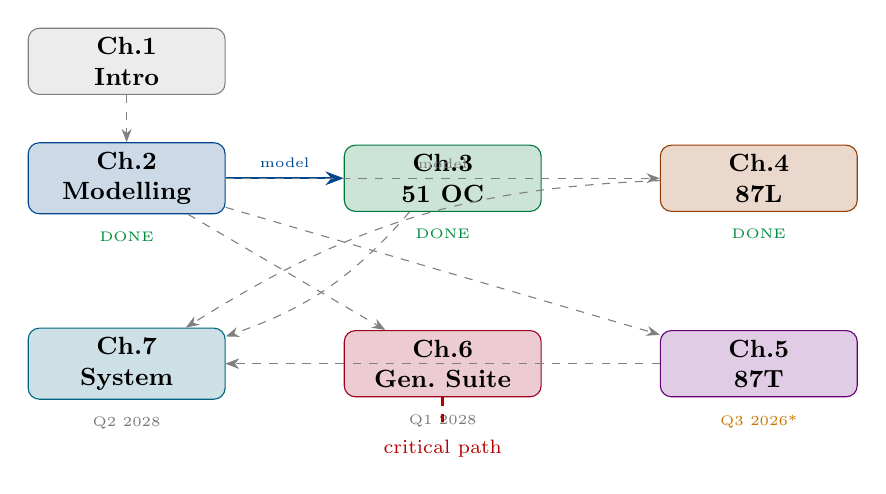
\begin{tikzpicture}[
  ch/.style={rectangle, draw, rounded corners, minimum width=2.5cm,
             minimum height=0.8cm, align=center, font=\small\bfseries},
  tr/.style={rectangle, draw, dashed, minimum width=2.2cm,
             minimum height=0.7cm, align=center, font=\scriptsize},
  arr/.style={-Stealth, thick},
  dep/.style={-Stealth, dashed, gray},
  node distance=0.8cm and 1.6cm,
]
% Chapters
\node[ch, fill=C1col!20, draw=C1col] (c2) {Ch.2\\Modelling};
\node[ch, fill=C2col!20, draw=C2col, right=1.5cm of c2] (c3) {Ch.3\\51 OC};
\node[ch, fill=C3col!20, draw=C3col, right=1.5cm of c3] (c4) {Ch.4\\87L};
\node[ch, fill=C4col!20, draw=C4col, below=1.5cm of c4] (c5) {Ch.5\\87T};
\node[ch, fill=C5col!20, draw=C5col, left=1.5cm of c5] (c6) {Ch.6\\Gen.\ Suite};
\node[ch, fill=C6col!20, draw=C6col, left=1.5cm of c6] (c7) {Ch.7\\System};
\node[ch, fill=gray!15, draw=gray, above=0.6cm of c2] (c1) {Ch.1\\Intro};

% Dependencies (must-read-before)
\draw[arr, C1col] (c2) -- node[above, font=\tiny]{model} (c3);
\draw[dep] (c2) -- node[above, font=\tiny]{model} (c4);
\draw[dep] (c2) -- (c5);
\draw[dep] (c2) -- (c6);
\draw[dep] (c3) to[bend left=15] (c7);
\draw[dep] (c4) to[bend right=15] (c7);
\draw[dep] (c5) -- (c7);
\draw[dep] (c6) -- (c7);
\draw[dep] (c1) -- (c2);

% Status badges
\node[below=0.1cm of c2, font=\tiny, donecol] {DONE};
\node[below=0.1cm of c3, font=\tiny, donecol] {DONE};
\node[below=0.1cm of c4, font=\tiny, donecol] {DONE};
\node[below=0.1cm of c5, font=\tiny, wip] {Q3 2026*};
\node[below=0.1cm of c6, font=\tiny, planned] {Q1 2028};
\node[below=0.1cm of c7, font=\tiny, planned] {Q2 2028};

% Critical path label
\draw[very thick, color=warningred, dashed] (c6.south) -- +(0,-0.4)
  node[below, font=\scriptsize, color=warningred] {critical path};
\end{tikzpicture}
\caption{Chapter dependency graph.  Solid arrows = strong prerequisite
(model used directly).  Dashed = logical dependency (motivation chain).
Ch.6 (generator suite) is the critical path: it gates Ch.7.}
\label{fig:dep}
\end{figure}

\textbf{Critical path:}
\begin{center}
TR-56 (Q3 2026) $\to$ TR-58/59/60/61 (Q1 2027) $\to$ TR-63/65 (Q4 2027)
$\to$ TR-66/67 (Q1 2028) $\to$ Ch.7 write-up (Q2 2028) $\to$ Submission (Q3 2028)
\end{center}

% ==============================================================================
\section{Gantt Timeline}
\label{sec:gantt}

\begin{figure}[!h]
\centering
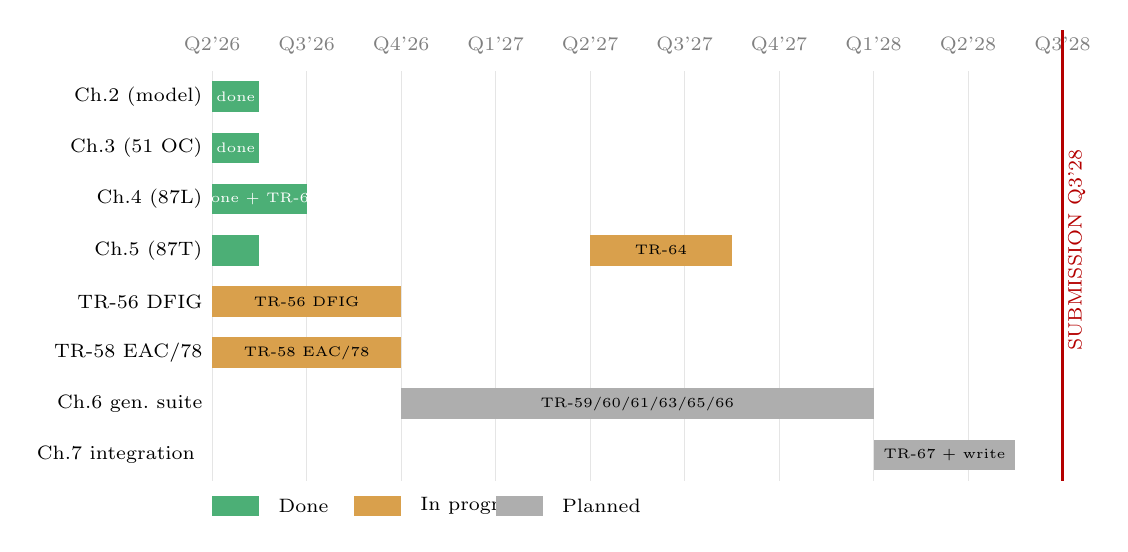
\begin{tikzpicture}[x=0.60cm, y=0.65cm]
% Grid
\foreach \q in {0,1,...,9} {
  \draw[gray!20, thin] (\q*2, -0.5) -- (\q*2, -8.5);
}
% Quarter labels
\foreach \q/\lbl in {0/Q2'26, 2/Q3'26, 4/Q4'26, 6/Q1'27, 8/Q2'27,
                      10/Q3'27, 12/Q4'27, 14/Q1'28, 16/Q2'28, 18/Q3'28} {
  \node[font=\scriptsize, gray] at (\q, 0) {\lbl};
}
% Row labels
\foreach \row/\lbl in {
  -1/{Ch.2 (model)},
  -2/{Ch.3 (51 OC)},
  -3/{Ch.4 (87L)},
  -4/{Ch.5 (87T)},
  -5/{TR-56 DFIG},
  -6/{TR-58 EAC/78},
  -7/{Ch.6 gen.\ suite},
  -8/{Ch.7 integration}
} {
  \node[left, font=\scriptsize, align=right] at (0, \row) {\lbl};
}
% Bars — [start, end, row, colour, label]
% Ch.2: done
\fill[donecol!70] (0,-1.3) rectangle (1,-0.7);
\node[font=\tiny, white] at (0.5,-1.0) {done};
% Ch.3: done
\fill[donecol!70] (0,-2.3) rectangle (1,-1.7);
\node[font=\tiny, white] at (0.5,-2.0) {done};
% Ch.4: done (+ TR-62 add-on Q2'26)
\fill[donecol!70] (0,-3.3) rectangle (2,-2.7);
\node[font=\tiny, white] at (1,-3.0) {done + TR-62};
% Ch.5: TR-57 done; TR-64 Q2-Q3 2027
\fill[donecol!70] (0,-4.3) rectangle (1,-3.7);
\fill[wip!70] (8,-4.3) rectangle (11,-3.7);
\node[font=\tiny] at (9.5,-4.0) {TR-64};
% TR-56
\fill[wip!70] (0,-5.3) rectangle (4,-4.7);
\node[font=\tiny] at (2,-5.0) {TR-56 DFIG};
% TR-58
\fill[wip!70] (0,-6.3) rectangle (4,-5.7);
\node[font=\tiny] at (2,-6.0) {TR-58 EAC/78};
% Ch.6 full
\fill[planned!60] (4,-7.3) rectangle (14,-6.7);
\node[font=\tiny] at (9,-7.0) {TR-59/60/61/63/65/66};
% Ch.7
\fill[planned!60] (14,-8.3) rectangle (17,-7.7);
\node[font=\tiny] at (15.5,-8.0) {TR-67 + write};
% Submission marker
\draw[very thick, color=warningred] (18, -8.5) -- (18, 0.3);
\node[color=warningred, font=\scriptsize, rotate=90] at (18.3, -4) {SUBMISSION Q3'28};
% Legend
\fill[donecol!70] (0,-9.2) rectangle (1,-8.8);
\node[right, font=\scriptsize] at (1.2,-9.0) {Done};
\fill[wip!70] (3,-9.2) rectangle (4,-8.8);
\node[right, font=\scriptsize] at (4.2,-9.0) {In progress};
\fill[planned!60] (6,-9.2) rectangle (7,-8.8);
\node[right, font=\scriptsize] at (7.2,-9.0) {Planned};
\end{tikzpicture}
\caption{Thesis Gantt chart.  Critical path runs through TR-56/58 (Q2--Q3 2026)
to the full generator suite (Q4 2027) and HIL validation (Q1 2028).}
\label{fig:gantt}
\end{figure}

% ==============================================================================
\section{Rules for New TRs}
\label{sec:rules}

Before starting any new TR (starting with TR-56), the following must be declared:

\begin{enumerate}
  \item \textbf{Chapter home.}  Which chapter does this TR feed?
    A TR that doesn't fit any chapter does not get written.

  \item \textbf{Section slot.}  Which §X.Y within that chapter?
    The chapter outline (Sections~\ref{sec:chapters}) defines all section slots.
    A new TR must either fill an existing slot or explicitly request a new slot
    (which requires justifying why the chapter outline was incomplete).

  \item \textbf{Unifying problem contribution.}  One sentence: what failure mode
    does this TR fix, and in which operating condition?  Must be distinct from
    all existing TRs.

  \item \textbf{Evidence standard.}  Minimum: one simulation validation study
    (deterministic or MC).  Maximum: PSCAD + HIL (deferred to TR-67).

  \item \textbf{Journal target.}  Which venue?  A TR without a journal target is
    an internal document only and does not count toward the publication tally.
\end{enumerate}

\textbf{TR-56 declaration (applying these rules):}
\begin{itemize}[nosep]
  \item Chapter: 6 (Generator Suite)
  \item Section slot: §6.1 (DFIG machine model for protection)
  \item Unifying problem: DFIG fault current has variable-amplitude slip-frequency
    DC that the 4-param SG model cannot fit — the 10-parameter piecewise ODE
    model is needed before any DFIG protection element can be designed
  \item Evidence: deterministic 10-scenario study + CUSUM crowbar detection test
  \item Journal: IEEE TEC
\end{itemize}

% ==============================================================================
\section{What This Map Does Not Include}
\label{sec:exclusions}

The following topics are explicitly \textbf{out of scope} and must not be added
to any chapter without a scope change review:

\begin{itemize}[nosep]
  \item Voltage ride-through (LVRT/HVRT) control — a generation problem, not protection
  \item Unit protection of PV strings or BESS internal faults — covered by IEEE 1547
  \item Cybersecurity of protection communications — not a relay-level problem
  \item Machine learning (ML) for protection — ruled out at thesis scoping stage
    (ML models have no IEC/IEEE standards path; physics-based estimators do)
  \item Market/economic optimisation of protection settings — different discipline
\end{itemize}

% ==============================================================================
\section{Summary Statistics}
\label{sec:stats}

\begin{table}[!h]
\centering
\caption{Thesis Statistics at Lock Date (April 2026)}
\label{tab:stats}
\begin{tabular}{lrr}
\toprule
Metric & Complete & Planned \\
\midrule
Technical reports (TRs) & 55 + 2 (TR-57, 62) = 57 & +10 (TR-56--67 minus done) \\
Journal papers complete & 4 (A, B, D, E) + partial (C, F) & +4 planned \\
Python modules (protection) & 12+ (line\_diff, sync\_oc suites) & +6--8 (generator suite) \\
Thesis pages written & $\sim$100 (Ch.3--4 + background) & +125 (Ch.5--7) \\
Published/submitted papers & 0 (none submitted yet) & 6 journal targets \\
MC trial count (to date) & 15k (87L) + 5k (SPRT plan) & +35k (generator suite) \\
\bottomrule
\end{tabular}
\end{table}

\end{document}
